\chapter{Diagramas E--pH}\label{ch:b1:e-ph-diagrams}

Un clavo de hierro abandonado en agua de lluvia se oxida; el mismo clavo
en una disolución muy básica conserva su brillo durante semanas. El casco
de acero de un barco lleva bloques de cinc que se disuelven en su lugar,
y un tejado de cobre se vuelve verde pero nunca desaparece. \omterm{def:b1:nernst:couple}{Pares redox}
cuyo potencial depende del pH, precipitación de hidróxidos y óxidos,
equilibrios ácido--base: los tres actúan a la vez, y un solo mapa los
reúne. En una gráfica del potencial frente al pH, cada especie de un
elemento recibe la región en la que es la forma estable; leer el mapa
dice qué especies sobreviven en el agua, cuáles reaccionan entre sí y
dónde se corroe un metal.

\begin{recall}
La \omterm{thm:b1:nernst:nernst}{ecuación de Nernst}, los \omterm{def:b1:nernst:electrode-potential}{potenciales estándar} y la predicción de las
reacciones redox están en el \cref{ch:b1:nernst}; los \omterm{def:b1:predominant-reaction:predominance}{diagramas de
predominio}, en el \cref{ch:b1:predominant-reaction}; los umbrales de
precipitación de los hidróxidos y los \omterm{def:b1:precipitation:existence-domain}{dominios de existencia} de los
sólidos, en el \cref{ch:b1:precipitation}. Todos los potenciales son a
\qty{25}{\celsius}, con $RT\ln 10/F = \qty{0.059}{V}$.
\end{recall}

\begin{omfigure}
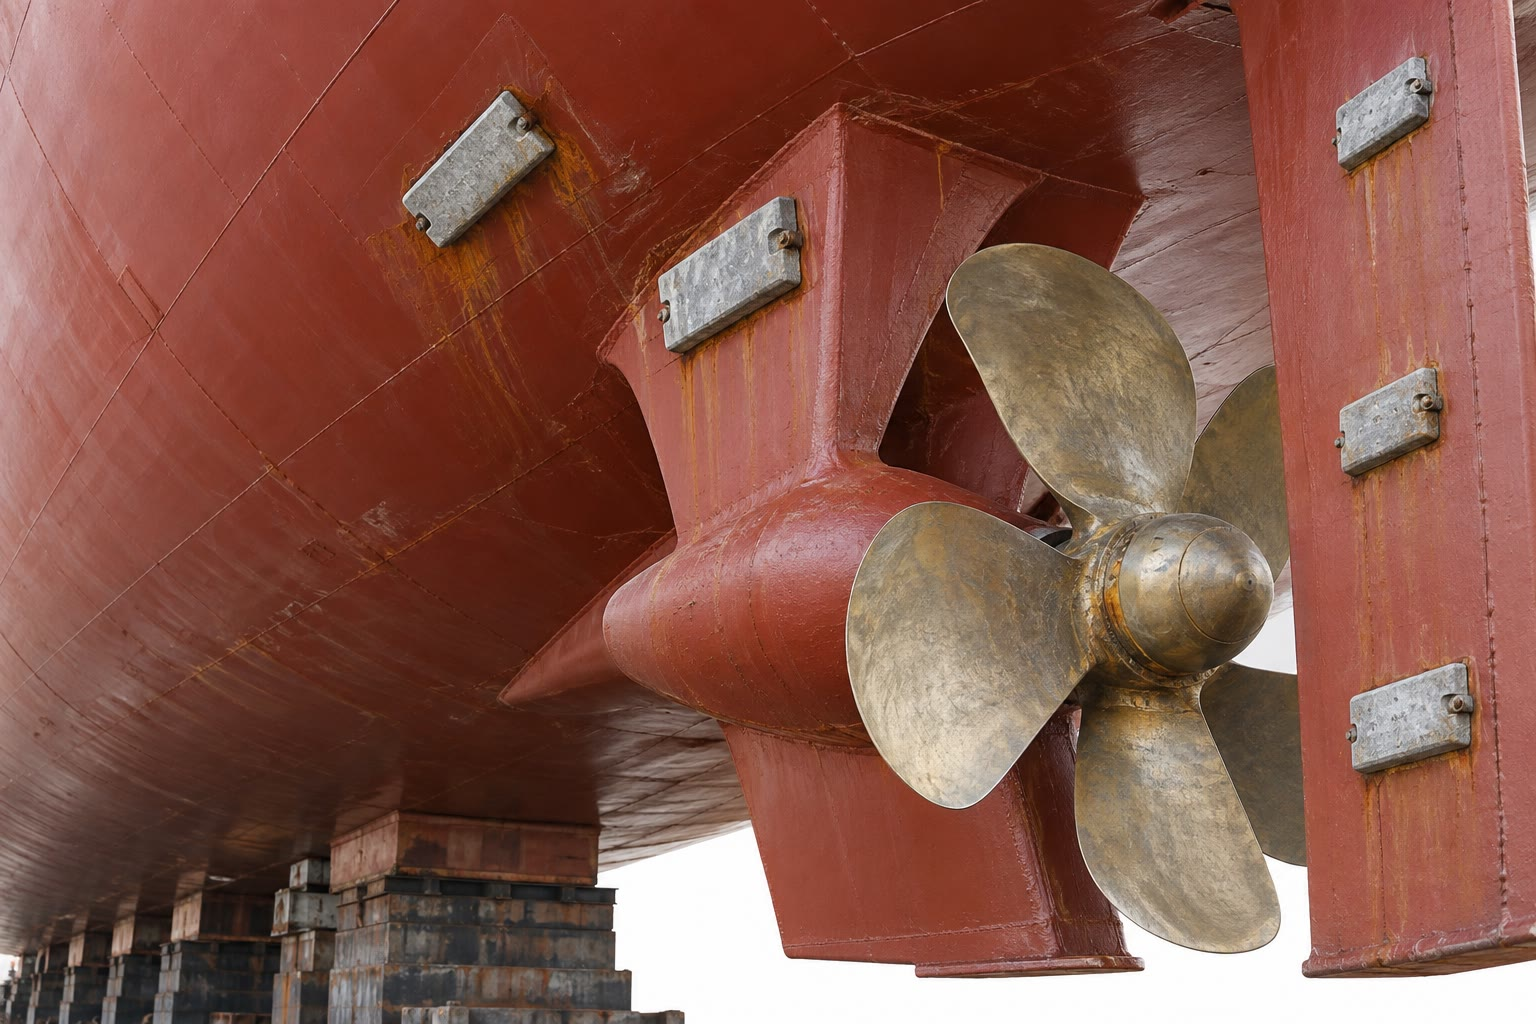
\includegraphics[width=0.6\linewidth]{images/book2/ai/b1-14-ship-anodes.jpg}

{\small La popa de un barco en dique seco. Los bloques grises fijados al
casco cerca de la hélice son de cinc: en el agua de mar se corroen en
lugar del acero (\cref{exo:b1:e-ph-diagrams:12}).}
\end{omfigure}

\section{Convenios}

\begin{definition}[Diagrama potencial--pH, concentración de trabajo]\label{def:b1:e-ph-diagrams:e-ph-diagram}
El \emph{diagrama potencial--pH}\index{diagrama potencial--pH} de un
elemento es el plano $(\mathrm{pH}, E)$ dividido en regiones, cada una de
las cuales es el dominio de predominio (especies disueltas) o de
existencia (sólidos) de una forma del elemento. Se traza para una
\emph{concentración de trabajo}\index{concentracion de trabajo@concentración de trabajo} $c$ elegida, la
concentración total del elemento en disolución, con estos convenios:
\begin{itemize}
  \item en una frontera entre dos especies disueltas, cada una está a $c$
        (contada en átomos del elemento);
  \item en una frontera entre una especie disuelta y un sólido, la
        especie disuelta está a $c$ y el sólido acaba de aparecer;
  \item los gases están a \qty{1}{bar}.
\end{itemize}
En este capítulo, $c = \qty{0.010}{mol/L}$.
\end{definition}

Las formas del elemento se ordenan por \omterm{def:b1:nernst:oxidation-number}{número de oxidación}: cuanto mayor
es el número, más arriba en el diagrama (las formas oxidadas son estables
a potencial alto). A igual \omterm{def:b1:nernst:oxidation-number}{número de oxidación}, las formas más básicas
(hidróxidos, óxidos, \omterm{def:b1:complexation:complex}{complejos} hidroxo) están a la derecha.

\begin{proposition}[Pendiente de una frontera]\label{prop:b1:e-ph-diagrams:boundary-slope}
Una frontera entre dos especies de \omterm{def:b1:nernst:oxidation-number}{números de oxidación} distintos, cuya
\omterm{def:b1:nernst:couple}{semiecuación} intercambia $n$ electrones y $m$ protones,
$\mathrm{Ox} + m\,\ce{H+} + n\,\mathrm{e^-} \rightleftharpoons \mathrm{Red} +
\cdots$, es una recta de pendiente $-0.059\,m/n$ voltios por unidad de
pH. Una frontera entre dos especies del mismo \omterm{def:b1:nernst:oxidation-number}{número de oxidación} es
vertical.
\end{proposition}

\begin{proof}
La \omterm{thm:b1:nernst:nernst}{ecuación de Nernst} da $E = E^\circ + \frac{0.059}{n}\log\frac{[\mathrm{Ox}]
[\ce{H+}]^m}{[\mathrm{Red}]} = E^\circ + \frac{0.059}{n}\log\frac{[\mathrm{Ox}]}
{[\mathrm{Red}]} - \frac{0.059\,m}{n}\,\mathrm{pH}$, y en la frontera las
concentraciones están fijadas por los convenios. Dos especies del mismo
\omterm{def:b1:nernst:oxidation-number}{número de oxidación} están relacionadas por un equilibrio ácido--base o de
precipitación sin electrones, cuya constante fija el pH de la frontera
sea cual sea el potencial.
\end{proof}

\section{El agua}

\begin{proposition}[Las dos rectas del agua]\label{prop:b1:e-ph-diagrams:water-lines}
Bajo \qty{1}{bar} de gas, el agua se reduce a hidrógeno por debajo de la
recta $E = -0.059\,\mathrm{pH}$ y se oxida a oxígeno por encima de la
recta $E = 1.23
- 0.059\,\mathrm{pH}$.
\end{proposition}

\begin{proof}
\ce{2H+ + 2e- -> H2}: $E = 0 + \frac{0.059}{2}\log\frac{[\ce{H+}]^2}{p(\ce{H2})}
= -0.059\,\mathrm{pH}$ con $p = 1$. \ce{O2 + 4H+ + 4e- -> 2H2O}: $E = 1.23 +
\frac{0.059}{4}\log(p(\ce{O2})[\ce{H+}]^4) = 1.23 - 0.059\,\mathrm{pH}$. Por
debajo de la primera recta, \ce{H2} es la forma estable del par (el agua
se reduce); por encima de la segunda, lo es \ce{O2}.
\end{proof}

\begin{definition}[Dominio de estabilidad del agua]\label{def:b1:e-ph-diagrams:water-domain}
La banda entre las dos rectas, de \qty{1.23}{V} de anchura a cualquier
pH, es el \emph{dominio de estabilidad del agua}\index{dominio de estabilidad del agua}:
una especie cuyo dominio está por completo dentro de ella ni oxida ni
reduce el agua.
\end{definition}

\section{Construcción de un diagrama: el hierro}

\begin{method}[Construir un diagrama potencial--pH]\label{met:b1:e-ph-diagrams:build}
\begin{enumerate}
  \item Se enumeran las especies y se ordenan por \omterm{def:b1:nernst:oxidation-number}{número de oxidación}:
        para el hierro, \ce{Fe} (0), \ce{Fe^2+} y \ce{Fe(OH)2} ($+$II),
        \ce{Fe^3+} y \ce{Fe(OH)3} ($+$III).
  \item En cada \omterm{def:b1:nernst:oxidation-number}{número de oxidación}, se hallan las fronteras verticales a
        partir de los equilibrios de precipitación (o ácido--base) a la
        \omterm{def:b1:e-ph-diagrams:e-ph-diagram}{concentración de trabajo} (\cref{ch:b1:precipitation}).
  \item Para cada par de \omterm{def:b1:nernst:oxidation-number}{números de oxidación} vecinos, se escribe la
        \omterm{def:b1:nernst:couple}{semiecuación} en cada intervalo de pH y su \omterm{thm:b1:nernst:nernst}{ecuación de Nernst} con
        los convenios; así se obtiene una frontera recta de pendiente
        conocida.
  \item Se ensamblan las rectas de izquierda a derecha; donde se cortan
        tres rectas, cada una continúa solo del lado en que sus dos
        especies son estables.
  \item Se comprueba: los dominios no deben solaparse, y las pendientes
        deben concordar con la
        \cref{prop:b1:e-ph-diagrams:boundary-slope}.
\end{enumerate}
\end{method}

\begin{example}[Las fronteras del hierro]\label{ex:b1:e-ph-diagrams:iron}
Con $c = \qty{0.010}{mol/L}$ (y las constantes de los \cref{ch:b1:precipitation,ch:b1:nernst}):
\begin{itemize}
  \item \ce{Fe^3+}/\ce{Fe(OH)3}: $\mathrm{pH} = 14.00 - \frac13(38.55 - 2) = 1.82$;
        \ce{Fe^2+}/\ce{Fe(OH)2}: $\mathrm{pH} = 14.00 - \frac12(16.31 - 2) = 6.85$.
  \item \ce{Fe^2+}/\ce{Fe}: $E = -0.41 + 0.030\log c = -0.47$~V (pH por
        debajo de 6.85).
  \item \ce{Fe^3+}/\ce{Fe^2+}: $E = 0.77$~V (ambos a $c$, pH por debajo de
        1.82).
  \item \ce{Fe(OH)3}/\ce{Fe^2+}: \ce{Fe(OH)3 + 3H+ + e- -> Fe^2+ + 3H2O},
        pendiente
        $-0.177$: $E = 1.09 - 0.177\,\mathrm{pH}$ entre pH 1.82 y 6.85.
  \item \ce{Fe(OH)3}/\ce{Fe(OH)2}: un electrón, un protón, $E = 0.28 -
        0.059\,\mathrm{pH}$; \ce{Fe(OH)2}/\ce{Fe}: dos electrones, dos
        protones, $E = -0.07 - 0.059\,\mathrm{pH}$ (pH por encima de
        6.85).
\end{itemize}
Las ordenadas en el origen se obtienen por continuidad en los puntos
triples, o directamente a partir de las entalpías libres de formación; el
diagrama de abajo se calcula a partir de estas últimas, y sus fronteras
difieren de estos valores redondeados en menos de \qty{0.01}{V} o de 0.01
unidades de pH.
% ledger: dfg:Fe2+_ao, dfg:Fe3+_ao, dfg:Fe_OH2_cr, dfg:Fe_OH3_cr, dfg:H2O_l, dfg:OH-_ao (boundaries computed in figdata/bachelor-1/eph-diagrams.py)
\end{example}

\begin{omfigure}
\begin{tikzpicture}
\begin{axis}[
  width=0.8\linewidth, height=8.2cm, xmin=0, xmax=14, ymin=-1.2, ymax=1.6,
  axis x line=bottom, axis y line=left, xlabel={pH}, ylabel={$E$ (V)},
  xtick={0,2,4,6,8,10,12,14}, ytick={-1,-0.5,0,0.5,1,1.5},
  unbounded coords=jump, clip=true,
  tick label style={font=\small}, label style={font=\small}]
\addplot[black!45, dashed] table[x=pH, y=H2] {figdata/out/bachelor-1-eph-diagrams-water.dat};
\addplot[black!45, dashed] table[x=pH, y=O2] {figdata/out/bachelor-1-eph-diagrams-water.dat};
\addplot[omDef, very thick] table[x=pH, y=E] {figdata/out/bachelor-1-eph-diagrams-iron.dat};
\node[font=\small] at (axis cs:3.2,-0.85) {\ce{Fe}};
\node[font=\small] at (axis cs:3.4,0.15) {\ce{Fe^2+}};
\node[font=\small] at (axis cs:0.9,1.45) {\ce{Fe^3+}};
\node[font=\small] at (axis cs:8.5,0.25) {\ce{Fe(OH)3}};
\node[font=\scriptsize] at (axis cs:11.0,-0.56) {\ce{Fe(OH)2}};
\node[font=\scriptsize, black!55, rotate=-14, anchor=south] at (axis cs:12.0,0.52) {\ce{O2}/\ce{H2O}};
\node[font=\scriptsize, black!55, rotate=-14, anchor=south] at (axis cs:2.2,-0.11) {\ce{H2O}/\ce{H2}};
\end{axis}
\end{tikzpicture}

{\small \omterm{def:b1:e-ph-diagrams:e-ph-diagram}{Diagrama potencial--pH} del hierro para $c = \qty{0.010}{mol/L}$
(líneas continuas), con las dos rectas del agua (discontinuas). Todas las
fronteras se calculan a partir de entalpías libres de formación
tabuladas.}
\end{omfigure}

\section{El cobre y el cinc}

El mismo método da los diagramas del cobre (especies \ce{Cu}, \ce{Cu+} y
\ce{Cu2O} en $+$I, \ce{Cu^2+} y \ce{CuO} en $+$II) y del cinc (\ce{Zn},
\ce{Zn^2+}, \ce{Zn(OH)2}, \ce{Zn(OH)4^2-}). Para el cobre, \ce{CuO}
aparece en $\mathrm{pH} = 14.00 - \frac12(20.64 - 2) = 4.68$, y el ion
\ce{Cu+}, aunque figura en la lista, no tiene ningún dominio: en medio
ácido, $E^\circ(\ce{Cu+}/\ce{Cu}) = 0.52$~V está por encima de
$E^\circ(\ce{Cu^2+}/\ce{Cu+}) = 0.16$~V, de modo que su supuesto dominio
queda tachado por sus dos vecinos (\cref{sec:b1:e-ph-diagrams:reading}).
Para el cinc, el hidróxido aparece a pH 6.81 y solo se redisuelve como
\ce{Zn(OH)4^2-} por encima de 13.97 a esta concentración, una franja
estrecha en el borde derecho.

\begin{omfigure}
\begin{tikzpicture}
\begin{axis}[name=cu,
  width=0.47\linewidth, height=7cm, xmin=0, xmax=14, ymin=-1.4, ymax=1.6,
  axis x line=bottom, axis y line=left, xlabel={pH}, ylabel={$E$ (V)},
  xtick={0,4,8,12}, ytick={-1,-0.5,0,0.5,1,1.5},
  unbounded coords=jump, clip=true,
  tick label style={font=\small}, label style={font=\small}]
\addplot[black!45, dashed] table[x=pH, y=H2] {figdata/out/bachelor-1-eph-diagrams-water.dat};
\addplot[black!45, dashed] table[x=pH, y=O2] {figdata/out/bachelor-1-eph-diagrams-water.dat};
\addplot[omDef, very thick] table[x=pH, y=E] {figdata/out/bachelor-1-eph-diagrams-copper.dat};
\node[font=\small] at (axis cs:5,-0.7) {\ce{Cu}};
\node[font=\small] at (axis cs:2,0.7) {\ce{Cu^2+}};
\node[font=\small] at (axis cs:9.5,0.75) {\ce{CuO}};
\node[font=\scriptsize] (cuo) at (axis cs:11.8,-1.05) {\ce{Cu2O}};
\draw[->, black!70] (cuo.north) -- (axis cs:10,-0.035);
\node[font=\small, anchor=north] at (axis cs:7,1.58) {cobre};
\end{axis}
\begin{axis}[at={(cu.east)}, anchor=west, xshift=1.5cm,
  width=0.47\linewidth, height=7cm, xmin=0, xmax=14, ymin=-1.4, ymax=1.6,
  axis x line=bottom, axis y line=left, xlabel={pH}, ylabel={$E$ (V)},
  xtick={0,4,8,12}, ytick={-1,-0.5,0,0.5,1,1.5},
  unbounded coords=jump, clip=true,
  tick label style={font=\small}, label style={font=\small}]
\addplot[black!45, dashed] table[x=pH, y=H2] {figdata/out/bachelor-1-eph-diagrams-water.dat};
\addplot[black!45, dashed] table[x=pH, y=O2] {figdata/out/bachelor-1-eph-diagrams-water.dat};
\addplot[omDef, very thick] table[x=pH, y=E] {figdata/out/bachelor-1-eph-diagrams-zinc.dat};
\node[font=\small] at (axis cs:3.5,-1.15) {\ce{Zn}};
\node[font=\small] at (axis cs:3.2,0.4) {\ce{Zn^2+}};
\node[font=\small] at (axis cs:10.2,0.4) {\ce{Zn(OH)2}};
\draw[->] (axis cs:12.4,1.15) node[left, font=\scriptsize] {\ce{Zn(OH)4^2-}} -- (axis cs:13.95,1.15);
\node[font=\small, anchor=north] at (axis cs:10.5,1.58) {cinc};
\end{axis}
\end{tikzpicture}

{\small \omterm{def:b1:e-ph-diagrams:e-ph-diagram}{Diagramas potencial--pH} del cobre y del cinc ($c =
\qty{0.010}{mol/L}$), con las rectas del agua (discontinuas). El dominio
del cobre metálico se solapa con el del agua; el del cinc está por
completo debajo de la recta del hidrógeno.}
% ledger: dfg:Cu+_ao, dfg:Cu2+_ao, dfg:Cu2O_cr, dfg:CuO_cr, dfg:Zn2+_ao, dfg:Zn_OH2_cr, dfg:Zn_OH42-_ao (boundaries computed in figdata/bachelor-1/eph-diagrams.py)
\end{omfigure}

\section{Leer un diagrama}\label{sec:b1:e-ph-diagrams:reading}

\begin{proposition}[Dominios disjuntos]\label{prop:b1:e-ph-diagrams:disjoint-domains}
Si, a un pH dado, el dominio de un \omterm{def:b1:nernst:couple}{oxidante} está por completo por encima
del de un \omterm{def:b1:nernst:couple}{reductor}, sin parte común, ambos reaccionan; las especies cuyos
dominios comparten una región pueden coexistir en equilibrio.
\end{proposition}

\begin{proof}
A ese pH, por encima de su frontera el par del \omterm{def:b1:nernst:couple}{oxidante} tiene un
potencial más alto que cualquiera que pueda alcanzar el par del \omterm{def:b1:nernst:couple}{reductor}:
según la \cref{prop:b1:nernst:equilibrium-constant}, la reacción entre
ellos tiene
$K > 1$ y continúa hasta que uno de los dos se agota o sus dominios se
encuentran. Dentro de una región común, ambos son las formas estables al
mismo potencial: nada impulsa una reacción.
\end{proof}

El hierro y el agua: el dominio del hierro metálico está por debajo de la
recta \ce{H2O}/\ce{H2} a cualquier pH. El hierro reduce el agua, en
disolución ácida con un desprendimiento visible de hidrógeno; con oxígeno
disuelto se oxida aún más deprisa. El cobre: su dominio se solapa con el
del agua, de modo que el cobre no reduce el agua ni los ácidos que no son
\omterm{def:b1:nernst:couple}{oxidantes}, pero el oxígeno del aire, situado por encima, lo oxida
lentamente --- la pátina verde de los tejados es un producto posterior de
esa oxidación con el dióxido de carbono y los compuestos de azufre. Un
diagrama dice lo que es posible, no a qué velocidad: muchas reacciones
que permite son lentas, una cuestión que se trata en el volumen del
segundo año.

\begin{definition}[Dismutación, comproporción]\label{def:b1:e-ph-diagrams:disproportionation}
La \emph{dismutación}\index{dismutacion@dismutación} es la reacción de una especie
consigo misma, en la que una parte se oxida y la otra se reduce:
\ce{2Cu+ -> Cu^2+ + Cu}. La reacción inversa, en la que dos especies del
mismo elemento dan una de \omterm{def:b1:nernst:oxidation-number}{número de oxidación} intermedio, es la
\emph{comproporción}\index{comproporcion@comproporción}:
\ce{2Fe^3+ + Fe -> 3Fe^2+}.
\end{definition}

\begin{proposition}[Criterio de dismutación]\label{prop:b1:e-ph-diagrams:disproportionation-criterion}
Una especie B de \omterm{def:b1:nernst:oxidation-number}{número de oxidación} intermedio, en los pares A/B y B/C,
se dismuta si $E(\mathrm{B}/\mathrm{C}) > E(\mathrm{A}/\mathrm{B})$:
entonces no tiene dominio propio, y una sola frontera A/C sustituye a las
dos.
\end{proposition}

\begin{proof}
B es el \omterm{def:b1:nernst:couple}{oxidante} de B/C y el \omterm{def:b1:nernst:couple}{reductor} de A/B. Si el par B/C está por
encima de A/B, la regla de la gamma (\cref{met:b1:nernst:predict-redox})
hace reaccionar B (\omterm{def:b1:nernst:couple}{oxidante}, par superior) con B (\omterm{def:b1:nernst:couple}{reductor}, par
inferior), dando C y A. Geométricamente, B solo sería estable por encima
de $E(\mathrm{B}/\mathrm{C})$ y por debajo de $E(\mathrm{A}/\mathrm{B})$,
un conjunto vacío.
\end{proof}

\begin{definition}[Dominios de inmunidad, de corrosión y de pasivación]\label{def:b1:e-ph-diagrams:corrosion-domains}
En el diagrama de un metal, el dominio del propio metal es su
\emph{dominio de inmunidad}\index{dominio de inmunidad} (no puede
oxidarse); los dominios de sus iones disueltos forman el \emph{dominio de
corrosión}\index{dominio de corrosion@dominio de corrosión}; los dominios de sus óxidos e
hidróxidos sólidos, que pueden recubrir el metal, forman el
\emph{dominio de pasivación}\index{dominio de pasivacion@dominio de pasivación}. Que un
recubrimiento proteja realmente el metal es una cuestión cinética, que se
trata en el volumen del segundo año.
\end{definition}

\begin{method}[Leer un diagrama]\label{met:b1:e-ph-diagrams:read}
\begin{enumerate}
  \item Se superponen las rectas del agua: una especie cuyo dominio está
        fuera de la banda del agua reacciona con el agua
        (termodinámicamente).
  \item Para dos especies de elementos distintos, se superponen sus
        diagramas: dominios disjuntos al pH de interés significan una
        reacción.
  \item Para un metal, se sitúa el punto (pH, $E$) del medio: inmunidad,
        corrosión o pasivación.
  \item Se recuerda que un diagrama se traza para una \omterm{def:b1:e-ph-diagrams:e-ph-diagram}{concentración de
        trabajo}; las fronteras con especies disueltas se desplazan
        $0.059/n$~V por década de concentración.
\end{enumerate}
\end{method}

El cinc protege el hierro: en el agua de mar (pH en torno a 8), el cinc y
el acero de un casco están en contacto; el cinc, de potencial más bajo,
se oxida primero, y los electrones que libera mantienen el hierro en su
\omterm{def:b1:e-ph-diagrams:corrosion-domains}{dominio de inmunidad} o cerca de él. El bloque de cinc se consume y se
sustituye en cada entrada en dique seco.

\section{Ejercicios}

\begin{exercise}[$\star$]\label{exo:b1:e-ph-diagrams:1}
Ordénense por \omterm{def:b1:nernst:oxidation-number}{número de oxidación} del elemento las especies \ce{Mn},
\ce{Mn^2+}, \ce{MnO2}, \ce{MnO4-}, \ce{Mn(OH)2}, y \ce{Cl-}, \ce{Cl2},
\ce{HClO},
\ce{ClO-}, \ce{ClO3-}.
\end{exercise}

\begin{exercise}[$\star$]\label{exo:b1:e-ph-diagrams:2}
Dese la pendiente de la frontera de cada \omterm{def:b1:nernst:couple}{semiecuación}:
\ce{Fe(OH)3 + 3H+ + e- -> Fe^2+ + 3H2O}; \ce{2Cu^2+ + H2O + 2e- -> Cu2O + 2H+};
\ce{MnO4- + 8H+ + 5e- -> Mn^2+ + 4H2O}; \ce{Zn(OH)2 + 2H+ + 2e- -> Zn + 2H2O}.
¿Por qué una de ellas tiene una pendiente positiva?
\end{exercise}

\begin{exercise}[$\star$]\label{exo:b1:e-ph-diagrams:3}
¿A qué pH pasan las rectas del agua por 0~V y por \qty{0.50}{V}? ¿Cuál es
la anchura del \omterm{def:b1:e-ph-diagrams:water-domain}{dominio de estabilidad del agua} a pH 7?
\end{exercise}

\begin{exercise}[$\star$]\label{exo:b1:e-ph-diagrams:4}
Con el diagrama del hierro, dese la forma estable del hierro en
(pH 1, $E = 1.0$~V), (pH 4, $E = 0$), (pH 10, $E = -0.4$~V) y
(pH 10, $E = 0.5$~V).
\end{exercise}

\begin{exercise}[$\star\star$]\label{exo:b1:e-ph-diagrams:5}
Recalcúlense la frontera \ce{Fe^2+}/\ce{Fe} y la vertical
\ce{Fe^3+}/\ce{Fe(OH)3} para una \omterm{def:b1:e-ph-diagrams:e-ph-diagram}{concentración de trabajo} de
\qty{1.0e-6}{mol/L}, el valor que se usa para discutir la corrosión. ¿Qué
dominios crecen?
\end{exercise}

\begin{exercise}[$\star\star$]\label{exo:b1:e-ph-diagrams:6}
Dedúzcase la frontera \ce{Fe(OH)3}/\ce{Fe^2+}: escríbanse la \omterm{def:b1:nernst:couple}{semiecuación}
y su \omterm{thm:b1:nernst:nernst}{ecuación de Nernst}, y úsese la continuidad en pH 1.82 para demostrar
que $E = 1.09 -
0.177\,\mathrm{pH}$.
\end{exercise}

\begin{exercise}[$\star\star$]\label{exo:b1:e-ph-diagrams:7}
Demuéstrese con la tabla de \omterm{def:b1:nernst:electrode-potential}{potenciales estándar} que \ce{Cu+} se dismuta
a pH 0, y dese el potencial de la frontera única \ce{Cu^2+}/\ce{Cu} para
$c = \qty{0.010}{mol/L}$.
\end{exercise}

\begin{exercise}[$\star\star$]\label{exo:b1:e-ph-diagrams:8}
¿Se disuelve el cobre en ácido clorhídrico a pH 0 sin aire? ¿Y en ácido
nítrico (par \ce{NO3-}/\ce{NO}, $E^\circ = 0.96$~V)? Justifíquese con el
diagrama y los potenciales.
\end{exercise}

\begin{exercise}[$\star\star$]\label{exo:b1:e-ph-diagrams:9}
Las disoluciones de hierro(II) que se dejan al aire se vuelven de color
pardo amarillento. Explíquese con el diagrama del hierro y la recta
\ce{O2}/\ce{H2O}, y escríbase la reacción a pH 3.
\end{exercise}

\begin{exercise}[$\star\star\star$]\label{exo:b1:e-ph-diagrams:10}
Constrúyase el diagrama del cinc para $c = \qty{0.010}{mol/L}$:
calcúlense las fronteras verticales en pH 6.81 y 13.97, la frontera
\ce{Zn^2+}/\ce{Zn} y las ecuaciones de \ce{Zn(OH)2}/\ce{Zn} y de
\ce{Zn(OH)4^2-}/\ce{Zn}.
\end{exercise}

\begin{exercise}[$\star\star\star$]\label{exo:b1:e-ph-diagrams:11}
Superpónganse los diagramas del hierro y del agua y discútase el destino
de un clavo de hierro en agua desoxigenada a pH 2, a pH 7 y a pH 13. ¿Qué
cambia con oxígeno disuelto?
\end{exercise}

\begin{exercise}[$\star\star\star$]\label{exo:b1:e-ph-diagrams:12}
\omterm{def:b1:nernst:cell}{Ánodos} de sacrificio. Un casco de acero en agua de mar (pH 8) está unido
a un bloque de cinc. Con los diagramas, explíquese qué metal se oxida,
escríbanse las reacciones con el oxígeno disuelto y dígase por qué el
magnesio también serviría y el cobre empeoraría las cosas.
\end{exercise}

\section{Problema: la lejía y la piscina}

\begin{problem}[{Problema de fin de semana --- los \omterm{def:b1:nernst:oxidation-number}{números de oxidación}
del cloro, el \omterm{def:b1:predominant-reaction:bronsted}{par ácido--base} HClO/ClO\textsuperscript{$-$}, el \omterm{def:b1:e-ph-diagrams:e-ph-diagram}{diagrama
potencial--pH} del cloro y el pH por encima del cual el cloro disuelto se
dismuta}]
\label{pb:b1:e-ph-diagrams:1}
La lejía es una disolución básica de hipoclorito de sodio y cloruro de
sodio; una piscina se desinfecta con el ácido hipocloroso que contiene,
con un pH mantenido algo por encima de 7. Mezclar lejía con un limpiador
ácido desprende cloro gaseoso. Datos a \qty{25}{\celsius}:
$E^\circ(\ce{Cl2(aq)}/\ce{Cl-})
= 1.396$~V, $E^\circ(\ce{HClO}/\ce{Cl2(aq)}) = 1.594$~V,
$\mathrm{p}K_a(\ce{HClO}/\ce{ClO-}) = 7.55$, $RT\ln 10/F = 0.0592$~V;
\omterm{def:b1:e-ph-diagrams:e-ph-diagram}{concentración de trabajo} $c = \qty{0.010}{mol/L}$ de átomos de cloro.

\medskip
\noindent\textbf{Parte I --- Las especies.}
\begin{enumerate}
  \item Dese el \omterm{def:b1:nernst:oxidation-number}{número de oxidación} del cloro en \ce{Cl-}, \ce{Cl2},
        \ce{HClO} y \ce{ClO-}.
  \item Ordénense las cuatro especies en un eje vertical de \omterm{def:b1:nernst:oxidation-number}{número de
        oxidación}.
  \item ¿Qué dos especies tienen el mismo \omterm{def:b1:nernst:oxidation-number}{número de oxidación}? ¿Qué
        relación hay entre ellas?
  \item Escríbase la \omterm{def:b1:nernst:couple}{semiecuación} de \ce{Cl2}/\ce{Cl-}.
  \item Escríbase la \omterm{def:b1:nernst:couple}{semiecuación} de \ce{HClO}/\ce{Cl2}.
  \item Escríbase la \omterm{def:b1:nernst:couple}{semiecuación} de \ce{ClO-}/\ce{Cl-} en disolución
        básica.
\end{enumerate}

\medskip
\noindent\textbf{Parte II --- El ácido hipocloroso.}
\begin{enumerate}[resume]
  \item Dibújese el \omterm{def:b1:predominant-reaction:predominance}{diagrama de predominio} de \ce{HClO} y \ce{ClO-} en
        función del pH.
  \item ¿Por qué es vertical su frontera en el \omterm{def:b1:e-ph-diagrams:e-ph-diagram}{diagrama potencial--pH}?
  \item Calcúlese la fracción de ácido hipocloroso a pH 7.4.
  \item Lo mismo a pH 8.0. El ácido hipocloroso es el mejor
        desinfectante: ¿por qué los encargados de las piscinas evitan que
        el pH suba hasta 8?
  \item En la lejía (pH en torno a 12), ¿qué forma está presente?
\end{enumerate}

\medskip
\noindent\textbf{Parte III --- El diagrama.}
Con los convenios del capítulo, en una frontera \ce{Cl2(aq)} está a $c/2$
y \ce{Cl-}, \ce{HClO} y \ce{ClO-}, a $c$.
\begin{enumerate}[resume]
  \item Demuéstrese que la frontera \ce{Cl2}/\ce{Cl-} está en $E = 1.396 +
        0.0296\log\bigl((c/2)/c^2\bigr) = 1.446$~V, independiente del pH.
  \item Demuéstrese que la frontera \ce{HClO}/\ce{Cl2} es $E = 1.594 -
        0.0296\log 50 - 0.0592\,\mathrm{pH} \approx 1.544 -
        0.0592\,\mathrm{pH}$.
  \item Hállese el pH en el que se cortan estas dos rectas.
  \item Más allá de ese pH, la frontera es \ce{HClO}/\ce{Cl-}. Escríbase su
        \omterm{def:b1:nernst:couple}{semiecuación} y demuéstrese que su pendiente es $-0.0296$.
  \item Calcúlese $E^\circ(\ce{HClO}/\ce{Cl-})$ a partir de los dos
        potenciales dados.
  \item Escríbase la frontera \ce{ClO-}/\ce{Cl-} por encima de pH 7.55;
        compruébese su continuidad en pH 7.55.
  \item Esbócese el diagrama de pH 0 a 14, con la recta \ce{O2}/\ce{H2O}.
  \item ¿Es estable termodinámicamente el ácido hipocloroso en el agua?
        ¿Por qué una piscina solo necesita, aun así, pequeñas adiciones
        diarias de cloro?
\end{enumerate}

\medskip
\noindent\textbf{Parte IV --- La \omterm{def:b1:e-ph-diagrams:disproportionation}{dismutación} y el peligro del ácido.}
\begin{enumerate}[resume]
  \item Por encima del pH de la pregunta 14, ¿qué le ocurre al cloro
        disuelto? Escríbase la reacción en agua y en disolución básica.
  \item ¿Cómo se fabrica la lejía a partir del cloro?
  \item Por debajo del mismo pH, escríbase la reacción entre \ce{HClO} y
        \ce{Cl-}. ¿Cómo se llama?
  \item Un limpiador ácido de inodoros lleva la lejía a pH 1. ¿Qué ocurre?
  \item ¿Por qué el peligro es menor con un producto débilmente ácido
        (pH 4)? Respóndase con el diagrama y, después, matícese.
  \item Dese, con un decimal, el pH por encima del cual el cloro disuelto
        se dismuta a $c = \qty{0.010}{mol/L}$.
\end{enumerate}
\end{problem}
